

\subsubsection{Tổng quan các dịch vụ của hệ thống}

\begin{figure}[H]
\centering
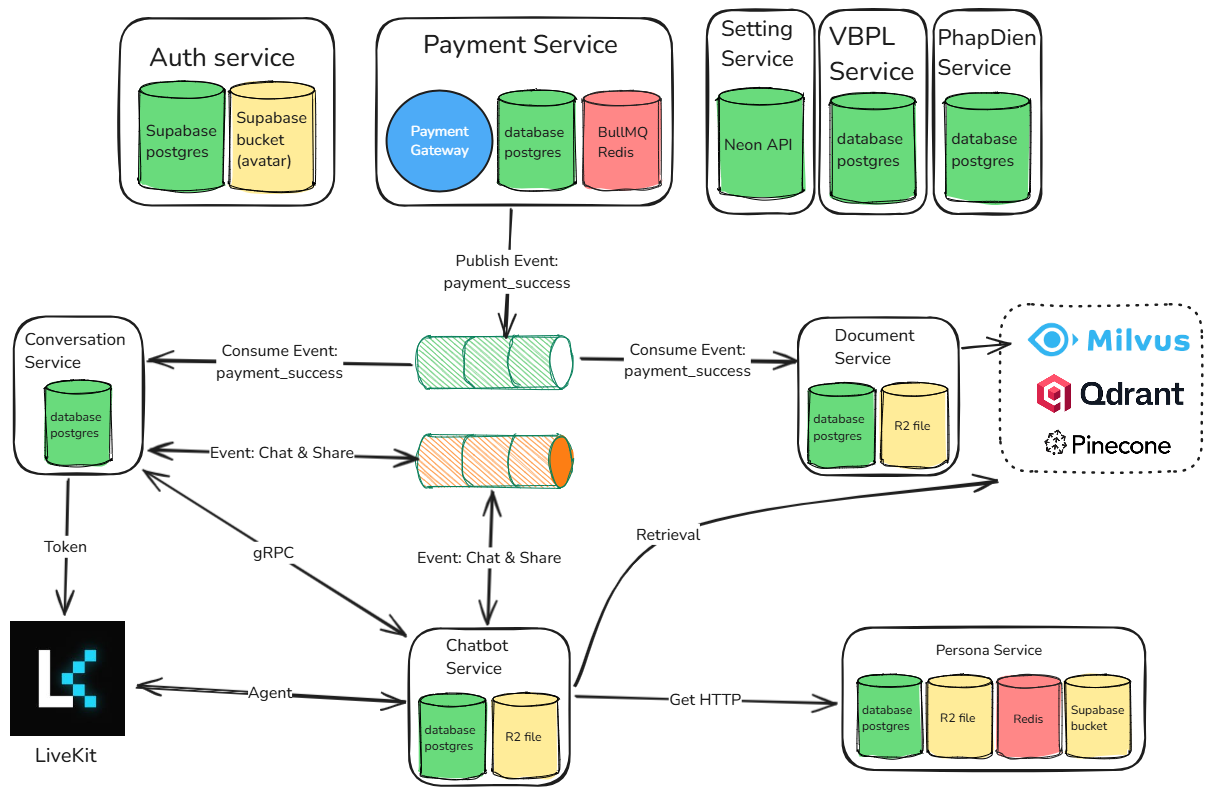
\includegraphics[width=0.95\textwidth]{pictures/Microservice-all.excalidraw.png}
\caption{Sơ đồ tổng quan các dịch vụ của hệ thống}
\end{figure}

Tất cả các dịch vụ đều dùng supabase để xác thực thông tin JWT của người dùng.
Tất cả các dịch vụ đều dùng CSDL Postgres của Neon để làm CSDL riêng theo đúng mẫu CSDL cho mỗi dịch vụ (database per service pattern). Mỗi dịch vụ sẽ sở hữu và quản lý hoàn toàn CSDL của riêng nó.

\begin{figure}[H]
\centering
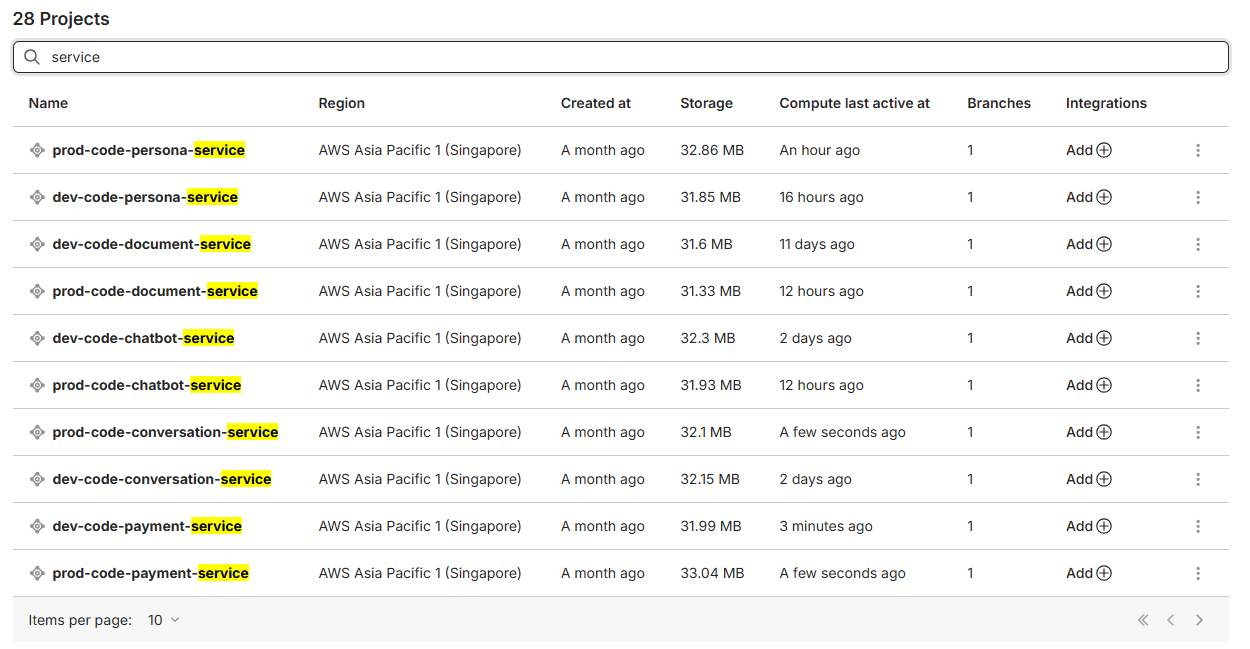
\includegraphics[width=0.95\textwidth]{pictures/neon-database-all.png}
\caption{Bảng điều khiển CSDL Neon}
\end{figure}

Các dịch vụ ngoại trừ auth
và setting được cấu hình
trong Kong API Gateway đơn giản
chỉ cần tạo Service và Route để định tuyến request.
Dịch vụ auth và setting sẽ được mô tả chi tiết
về cách cấu hình Kong API Gateway
trong nội dung trình bày của chính dịch vụ đó.
Vì trang thống kê thông tin
đường ống dữ liệu (Data Pipeline)
dành cho quản trị viên (ADMIN)
có tần suất truy vấn thấp
nên sẽ được triển khai trên Vercel.

\begin{figure}[H]
\centering
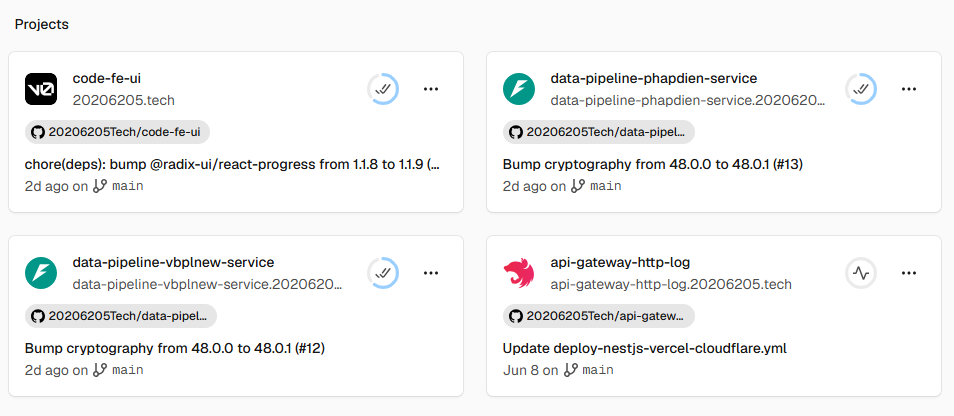
\includegraphics[width=0.95\textwidth]{pictures/vercel-project.png}
\caption{Bảng điều khiển các dự án trên Vercel}
\end{figure}

Các dịch vụ NestJS sử dụng Codecov để theo dõi độ bao phủ kiểm thử (test coverage).

\begin{figure}[H]
\centering
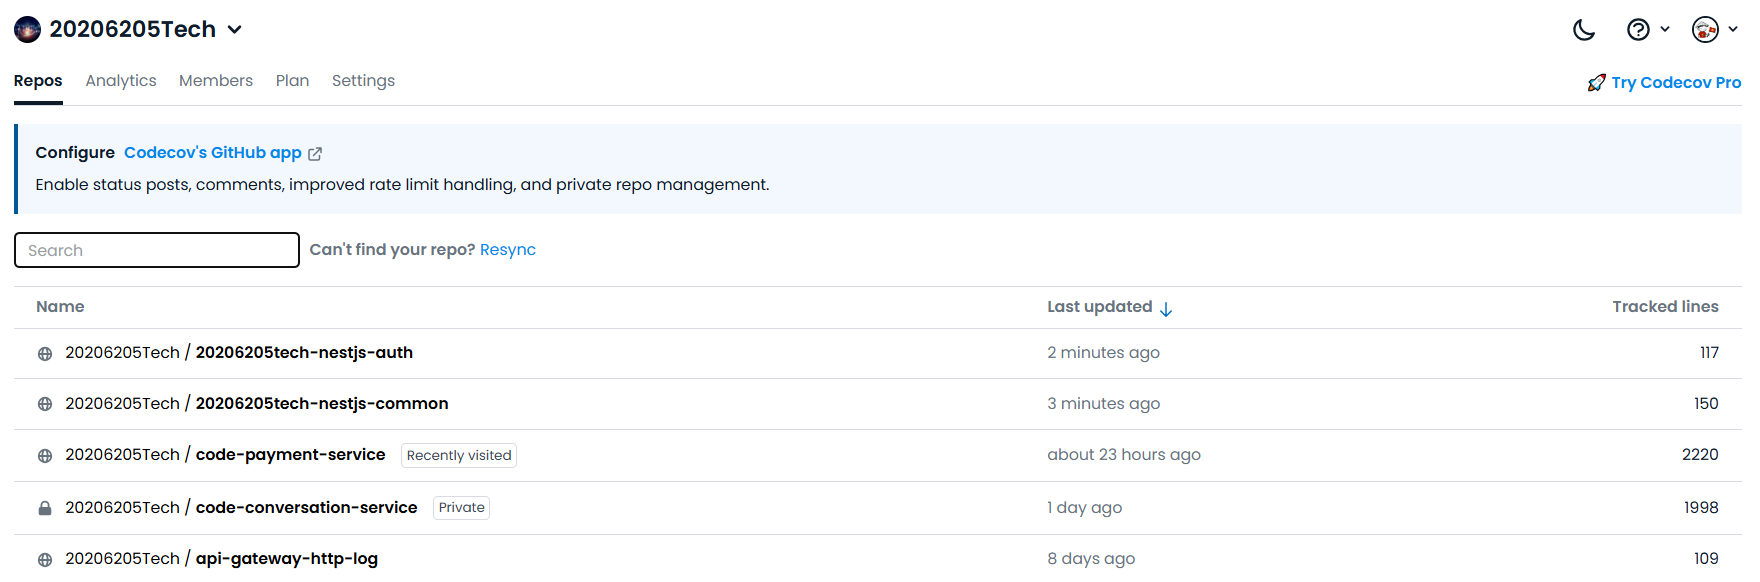
\includegraphics[width=0.95\textwidth]{pictures/test-codecov2.png}
\caption{Thống kê độ bao phủ kiểm thử trên CodeCov}
\end{figure}

Tích hợp SonarQube để phân tích chất lượng mã nguồn và các lỗ hổng bảo mật.

\begin{figure}[H]
\centering
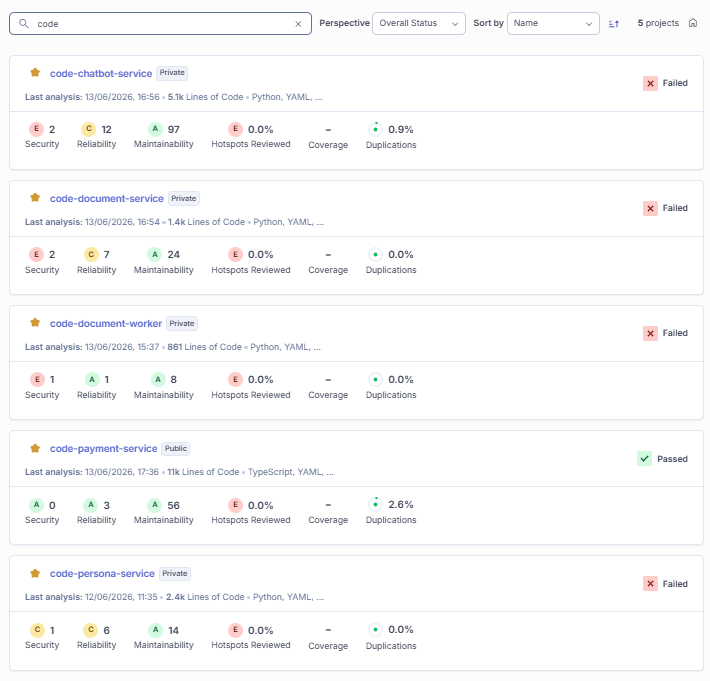
\includegraphics[width=0.95\textwidth]{pictures/sonarqube.png}
\caption{Giao diện phân tích mã nguồn trên SonarQube}
\end{figure}

% \subsubsection{Tracing và Quan sát hệ thống (Observability)}
% Hệ thống sử dụng \textbf{OpenTelemetry (OTel)} tích hợp trong tất cả các dịch vụ để tự động thu thập dấu vết phân tán (distributed traces) và gửi dữ liệu về Honeycomb.
Hệ thống
tích hợp Honeycomb để theo dõi vết (distributed tracing) giữa các dịch vụ.

\begin{figure}[H]
\centering
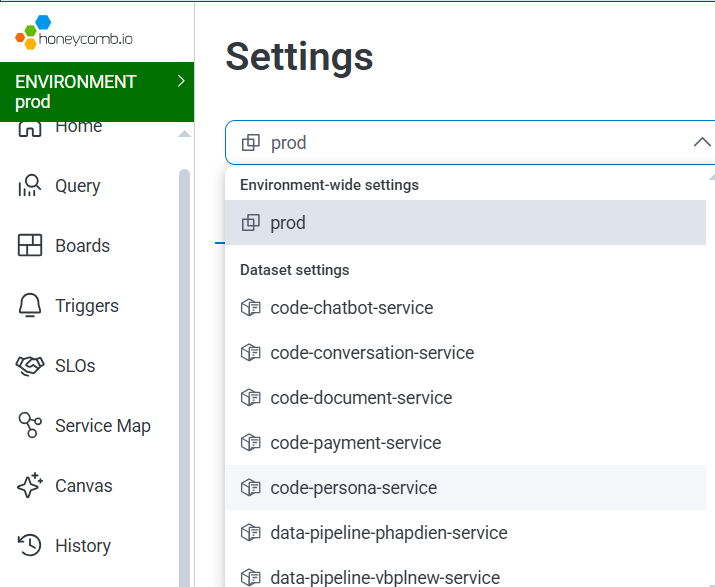
\includegraphics[width=0.95\textwidth]{pictures/tracing.png}
\caption{Giao diện theo dõi vết distributed tracing trên Honeycomb}
\end{figure}
